\documentclass[
11pt,%
tightenlines,%
twoside,%
onecolumn,%
nofloats,%
nobibnotes,%
nofootinbib,%
superscriptaddress,%
noshowpacs,%
centertags]%
{revtex4}
\usepackage{ljm}
\usepackage{listings}

\lstset{
language=C++,
basewidth=0.5em,
xleftmargin=45pt,
xrightmargin=45pt,
basicstyle=\small\ttfamily,
keywordstyle=\bfseries\underbar,
numbers=left,
numberstyle=\tiny,
stepnumber=1,
numbersep=10pt,
showspaces=false,
showstringspaces=false,
showtabs=false,
frame=trBL,
tabsize=2,
captionpos=t,
breaklines=true,
breakatwhitespace=false,
escapeinside={\%*}{*)}
}

\begin{document}

\titlerunning{short name}
\authorrunning{A.~A.~Rybakov and ...}

\title{Title\\Title}

\author{\firstname{A.~A.}~\surname{Rybakov}}
\email[E-mail: ]{rybakov.aax@gmail.com}
\affiliation{Joint Supercomputer Center of the Russian Academy of Sciences -- branch of Scientific Research Institute of System Analysis of the Russian Academy of Sciences, Leninsky prospect 32a, Moscow, 119334, Russia}

\firstcollaboration{(Submitted by S.~S.~Submitter)}

\received{April 01, 2020}

\begin{abstract}
Abstract.
\end{abstract}

\subclass{} % Enter 2010 Mathematics Subject Classification.

\keywords{Keyword1, keyword2.}

\maketitle

\section{Introduction}

Introduction.

\section{Section1}

Section1.
     
\section{Section2}

Section2.

\section{Section3}

Section3.

\begin{figure}[h]
\setcaptionmargin{5mm}
%\onelinecaptionsfalse % if the caption is multiline
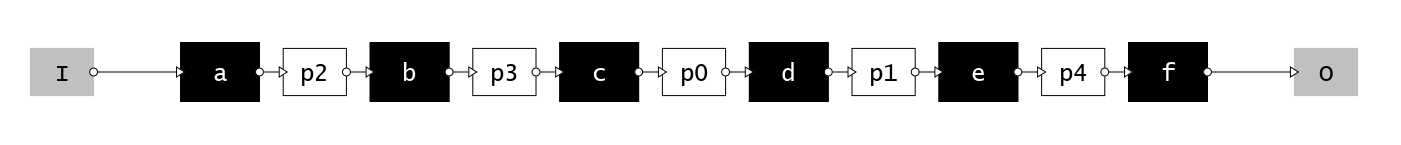
\includegraphics[width=0.95\textwidth]{pics/origin1.png}
\captionstyle{normal}\caption{Caption.}
\label{fig:origin1}
\end{figure}

\begin{figure}[h]
\setcaptionmargin{5mm}
%\onelinecaptionsfalse % if the caption is multiline
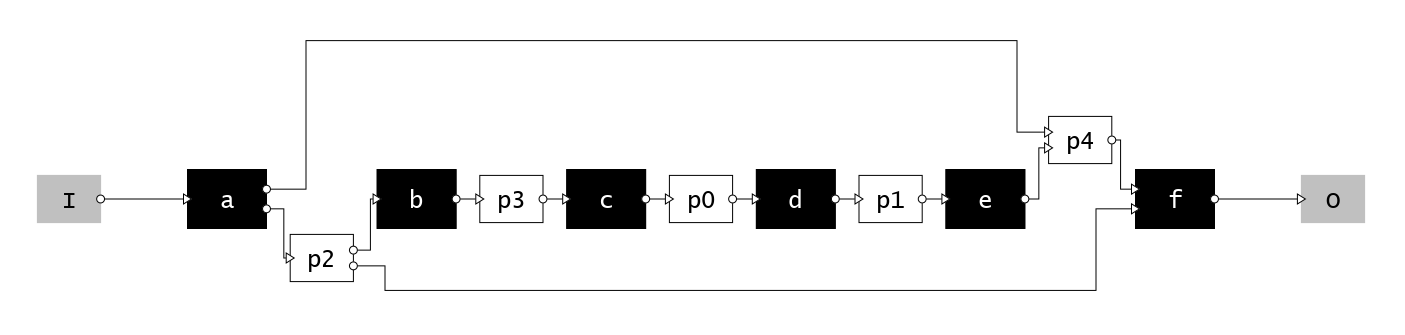
\includegraphics[width=0.95\textwidth]{pics/second1.png}
\captionstyle{normal}\caption{Caption.}
\label{fig:second1}
\end{figure}

\begin{figure}[h]
\setcaptionmargin{5mm}
%\onelinecaptionsfalse % if the caption is multiline
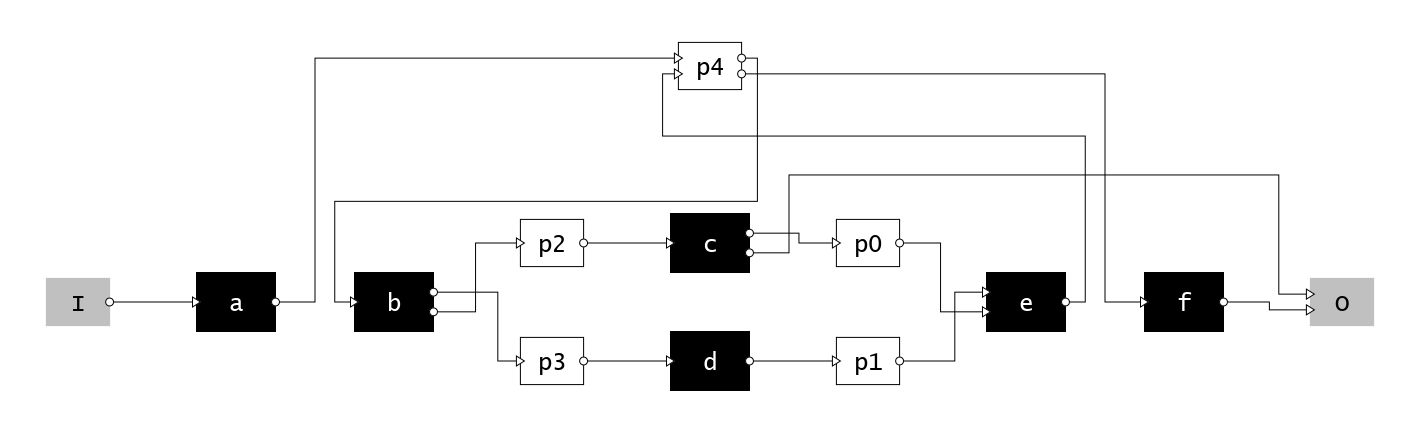
\includegraphics[width=0.95\textwidth]{pics/third1.png}
\captionstyle{normal}\caption{Caption.}
\label{fig:third1}
\end{figure}

\section{Conclusion}

Conclusion.

\begin{acknowledgments}
The work has been done at the JSCC RAS as part of the state assignment for the topic ... The supercomputer MVS-10P, located at the JSCC RAS, was used for calculations during the research.
\end{acknowledgments}

\begin{thebibliography}{99}

\bibitem{Rettinger}
\refitem{article}
C. Rettinger, C. Godenschwager, S. Eibl, et al., {\it ``Fully Resolved Simulations of Dune Formation in Riverbeds"}, ISC High Performance , LNCS~{\bf 10266}, 3--21 (2017).

\end{thebibliography}

\end{document}
